\documentclass[12pt, titlepage]{article}

\usepackage{booktabs}
\usepackage{tabularx}
\usepackage{hyperref}
\usepackage{comment}
\usepackage{graphicx}
\hypersetup{
    colorlinks,
    citecolor=blue,
    filecolor=black,
    linkcolor=red,
    urlcolor=blue
}
\usepackage[round]{natbib}

%% Comments

\usepackage{color}

\newif\ifcomments\commentstrue %displays comments
%\newif\ifcomments\commentsfalse %so that comments do not display

\ifcomments
\newcommand{\authornote}[3]{\textcolor{#1}{[#3 ---#2]}}
\newcommand{\todo}[1]{\textcolor{red}{[TODO: #1]}}
\else
\newcommand{\authornote}[3]{}
\newcommand{\todo}[1]{}
\fi

\newcommand{\wss}[1]{\authornote{blue}{SS}{#1}} 
\newcommand{\plt}[1]{\authornote{magenta}{TPLT}{#1}} %For explanation of the template
\newcommand{\an}[1]{\authornote{cyan}{Author}{#1}}

%% Common Parts

\newcommand{\progname}{OAR} % PUT YOUR PROGRAM NAME HERE
\newcommand{\authname}{Hunter Ceranic} % AUTHOR NAMES                  

\usepackage{hyperref}
    \hypersetup{colorlinks=true, linkcolor=blue, citecolor=blue, filecolor=blue,
                urlcolor=blue, unicode=false}
    \urlstyle{same}
                                


\newcounter{testnum} %Definition Number
\newcommand{\tthetestnum}{T\thetestnum}
\newcommand{\tref}[1]{T\ref{#1}}

\DeclareGraphicsExtensions{.bmp, .png, .jpg}

\begin{document}

\title{Optical Alphabet Recognition: System Verification and Validation Plan for \progname{OAR}} 
\author{Hunter Ceranic}
\date{February 19, 2024}
	
\maketitle

\pagenumbering{roman}

\section*{Revision History}

\begin{tabularx}{\textwidth}{p{3cm}p{2cm}X}
\toprule {\bf Date} & {\bf Version} & {\bf Notes}\\
\midrule
February 19, 2024 & 1.0 & Initial Revision\\
\bottomrule
\end{tabularx}

~\\
\wss{The intention of the VnV plan is to increase confidence in the software.
However, this does not mean listing every verification and validation technique
that has ever been devised.  The VnV plan should also be a \textbf{feasible}
plan. Execution of the plan should be possible with the time and team available.
If the full plan cannot be completed during the time available, it can either be
modified to ``fake it'', or a better solution is to add a section describing
what work has been completed and what work is still planned for the future.}

\wss{The VnV plan is typically started after the requirements stage, but before
the design stage.  This means that the sections related to unit testing cannot
initially be completed.  The sections will be filled in after the design stage
is complete.  the final version of the VnV plan should have all sections filled
in.}

\newpage

\tableofcontents

\listoffigures

\newpage

\section{Symbols, Abbreviations, and Acronyms}

\renewcommand{\arraystretch}{1.2}
\begin{tabular}{l l} 
  \toprule		
  \textbf{symbol} & \textbf{description}\\
  \midrule 
  R & Requirement\\
  SRS & System Requirements Specification\\
  T & Test\\
  VnV & Verification and Validation\\
  OAR & Optical Alphabet Recognition\\
  \bottomrule
\end{tabular}\\

\newpage

\pagenumbering{arabic}

This document describes the Verification and Validation plan for the OAR Project. Testing of the Software and its components
will be conducted in accordance with this document to improve confidence in the accuracy, understandibility and ability for the software 
to meet the requirements laid out in the Software Requirement Specifications (SRS).

\section{General Information}

\subsection{Summary}

The OAR project will result in software that is able to accurately classify input images of capital-letter English alphabet charcters using
logistic regression. An emphasis is placed on understandable code so that OAR can be a launch point for learning about optical
character recognition.

\subsection{Objectives}

The objective is to build confidence in the correctness of the software, and making sure it is comparable
to similar soultions (\textit{accuracy}). The correctness of the output is very easy for a user to evaluate themselves, so
it is essential the OAR project not only outputs the correct label, but is able to do so at a high confidence probability level.  
As a secondary goal, the \textit{understandability} of the code is important, as the project is designed as a learning tool.
This goal is a subset of making the code \textit{maintainable}, and will require both thorough code writing during implementation
and user input to validate. Parts of the code will rely on external libraries for operations like pre-processing input images,
however while it would be beneficial to verify the correctness of these libraries, this is out of the scope of the project and it will 
be assumed these external libraries will have been verified by their implementation teams.

\subsection{Relevant Documentation}

There are multiple design documents that provide in-depth details for understanding
the program being tested. These are as follows:

\begin{itemize}
  \item Problem Statement \citep{Prob_Statement}: States the problem we are trying to solve
    and introduces the topics that will need be verified.
  \item SRS \citep{SRS}: States the requirements, assumptions, models, and important 
  terminology that are used in the VnV plan.
  \item VnV Report \citep{VnV_report}: States what has been achieved from the VnV plan,
    and provides results or evidence to help build confidence for correctness.
  \item MG \citep{MG}: States the responsibilities and secrets for each module that will
    be evaluated by the VnV plan.
  \item MIS \citep{MIS}: Specifies the functional design and states what is needed for each
    module that will be evaluated by the VnV plan.
\end{itemize}

\section{Plan}

In this section, multiple plans are described to test and inspect the software with an emphasis 
on \textit{accuracy} and \textit{understandability}. Multiple approaches and perspectives will be employed by the VnV team (Section 3.1)
to help build confidence in the requirements, to avoid any missed important details, 
and to deliver on the outlined objectives (Section 2.2).

\subsection{Verification and Validation Team}

The members of the VnV team as well their individual roles are listed in the following table:

\begin{table}[h!]
  \centering
  \begin{tabular}{|r|l|}
    \hline
    \textbf{Role} & \textbf{Name} \\ \hline
    Project Supervisor & Dr.\ Spencer Smith  \\ \hline
    Author             & Hunter Ceranic      \\ \hline
    Domain Expert      & Adrian Sochaniwsky  \\ \hline
    SRS Reviewer       & Phil Du             \\ \hline
    VnV Plan Reviewer  & Goafeng Zhou        \\ \hline
    MG + MIS Reviewer  & Yiding Li           \\ \hline
  \end{tabular}
  \caption{Table of the VnV Team Members}
  \label{table_vnv_team}
\end{table}

\subsection{SRS Verification Plan}

The SRS will be reviewed by the project supervisor, the SRS reviewer and the author. Some input
may be given by the expert consultants if time permits. Most of the feedback has been provided 
through issues on GitHub, as annotated documents, or by verbal exchange. 
Throughout the development of the project, the author is expected 
to make changes needed to the resolve the issues. The reviewers may refer to the SRS checklist \citep{SRS_checklist}.
The key objective is to verify that the software requirements and the documentation are sound 
and coherent to the intended audience as defined in the SRS.

\subsection{Design Verification Plan}

Design decisions were made with a focus on performance and code understandability, so that the program could also be used 
as an educational tool for learning about image recognition. The design and implementation is documented in the 
MG\citep{MG}/MIS\citep{MIS} which will be verified with the MG \cite{MG_checklist}
and MIS \cite{MIS_checklist} checklists.
The VnV team will provide their input using these checklists through GitHub issues. 

\subsection{Verification and Validation Plan Verification Plan}

The goal is to uncover any mistakes and reveal any risks (such as misconceptions or coverage gaps) 
through the supervision and 
review of the VnV team members. Once most of the work has been done, the work and
accompanying documentation shall undergo a vetting process: the VnV team
will check whether the documented testing plans and verification process have been 
accomplished and the requirements fulfilled. The author will then review the documents
against the VnV checklist \citep{VnV_checklist}, before a final review by the rest of the VnV team.

\subsection{Implementation Verification Plan}

Both automated and manual testing will be performed for this project. This will include checking for any inconsistencies,
unexpected outputs, or bugs that may be encountered.
For all the code implemented linters and coverage tools will be implemented as described in Section 3.6. Furthermore,
tests for the program based on requirements will be performed using an automated test suite. Manual tests will be 
performed to benchmark the performance of the OAR project against already existing solutions.


\subsection{Automated Testing and Verification Tools}

Continous integration will be implemented for this project using CircleCI, which 
is easily integrated with GitHub and Python the programming language for the project. CircleCI automates the testing 
pipeline for the project, by running tests created using the pytest library and code coverage tests using the coverage.py library, 
on selected pushes or pulls to the repository. The test created with pytest are performed by predetermining potential user
inputs and comparing them with expected values. In addition to the continous integration suite, Flake 8 will be used as a 
linter for the code created through the VSCode IDE.

\subsection{Software Validation Plan}

Software validation is beyond the scope of the OAR project due to the sheer amount of experimental data needed to be collected to 
validate the system behaviour not being feasible, given the time constraints.

\section{System Test Description}
	
\subsection{Tests for Functional Requirements}

In this section, the system tests that will be conducted are described in detail. These tests
will be used to verify the fulfillment of the requirements as listed in the SRS \citep{SRS}.
Most, if not all, of the tests listed here will be automatically performed unless otherwise stated.

\subsubsection{Input Image Type}

To satisfy R1 from the SRS \citep{SRS}, any input image of the following formats listed below shall be 
accepted provided they follow the input data constraints.

\begin{itemize}
  \item{PNG}
  \item{JPG}
  \item{BMP\\}
\end{itemize}

\begin{enumerate}

  \item{\textbf{T\refstepcounter{testnum}\thetestnum \label{T_inputImage}}: Test input for PNG/JPG/BMP format\\}
            
  Control: Automatic
            
  Initial State: OAR loaded and idle.
            
  Input: A set of non-corrupt (valid) PNG, JPG, and BMP image files depicting valid label characters (see \ref{Fig_A}).
            
  Output: The predicted label should match the actual label as assigned by the oracle (the author).
            
  Test Case Derivation: These are some of the most common image file formats and should be compatible with the software.
            
  How test will be performed: The automatic test will be performed using pytest, executed by CircleCI.
\end{enumerate}

\subsubsection{Unprocessed Input Images}
To satisfy R2 from the SRS \citep{SRS}, regardless of colorscale or pixel size any input image should be able to be accepted to 
be processed into a format usable by the program. In addition, pixel sizes are constrained to the following ranges:

\begin{itemize}
  \item{\textit{max}: 4096px $\times$ 4096px}
  \item{\textit{min}: 20px $\times$ 20px}
\end{itemize}

\begin{enumerate}

  \item{\textbf{T\refstepcounter{testnum}\thetestnum \label{T_inputColour}}: Test input for images with different colour schemes\\}
            
  Control: Automatic
            
  Initial State: OAR loaded and idle.
            
  Input: A set of non-corrupt (valid) image files depicting valid label characters in black and white(\ref{Fig_BWA}), 
  grayscale (\ref{Fig_grayA}), red (\ref{Fig_redA}), green (\ref{Fig_greenA}) and blue (\ref{Fig_blueA}).
  
  Output: The predicted label should match the actual label as assigned by the oracle (the author).
            
  Test Case Derivation: These images cover the cases of greyscale, black and white and RGB images which should be compatible with the software.
            
  How test will be performed: The automatic test will be performed using pytest, executed by CircleCI.

  \item{\textbf{T\refstepcounter{testnum}\thetestnum \label{T_inputSize}}: Test input for images with different pixel sizes\\}
            
  Control: Automatic
            
  Initial State: OAR loaded and idle.
            
  Input: A set of non-corrupt (valid) image files depicting valid label characters (see \ref{Fig_A}) of the following sizes:
  \begin{itemize}
    \item{8192px $\times$ 8192px}
    \item{4096px $\times$ 4096px}
    \item{1024px $\times$ 1024px}
    \item{20px $\times$ 20px}
    \item{10px $\times$ 10px}
  \end{itemize}
            
  Output: In the 8192px $\times$ 8192px and 10px $\times$ 10px cases the program should provide the user with an error. In all other cases,
  the predicted label should match the actual label as assigned by the oracle (the author).
            
  Test Case Derivation: These images cover the range of acceptable pixel sizes, as well as outside of the range which should be compatible with the software.
            
  How test will be performed: The automatic test will be performed using pytest, executed by CircleCI.
\end{enumerate}

\subsubsection{Output Labels}

To satisfy R4 (and by extension R3) from the SRS \citep{SRS}, any input image should be properly classified and related to the 
correct output label from the set of 26 letters: {A,B,C,D,E,F,G,H,I,J,K,L,M,N,O,P,Q,R,S,T,U,V,W,X,Y,Z}

\begin{enumerate}

  \item{\textbf{T\refstepcounter{testnum}\thetestnum \label{T_outputLabel}}: Test input for images with different pixel sizes\\}
            
  Control: Automatic
            
  Initial State: OAR loaded and idle.
            
  Input: A set of non-corrupt (valid) image files depicting all 26 valid label characters(\ref{Fig_A}), and a blank image depicting no character (\ref{Fig_blank}).
            
  Output: The predicted label output should match the actual label as assigned by the oracle (the author). The output for the blank image
  should state "No Label Detected".
            
  Test Case Derivation: These images cover the range of possible label outputs for the program.
            
  How test will be performed: The automatic test will be performed using pytest, executed by CircleCI.
\end{enumerate}

\subsubsection{Output Label Confidence Level}

To satisfy R5 from the SRS \citep{SRS}, any classified input image should also have an associated valid confidence level in the range of
0-100\%.

\begin{enumerate}

  \item{\textbf{T\refstepcounter{testnum}\thetestnum \label{T_outputConf}}: Test input for images with different pixel sizes\\}
            
  Control: Automatic
            
  Initial State: OAR loaded and idle.
            
  Input: A set of non-corrupt (valid) image files depicting an input character from the training set, an input character from the test set,
  an image depicting multiple characters and a blank image depicting no characters.
            
  Output: For each case the outputs would be as follows:
  \begin{itemize}
    \item{Training Set Image (\ref{Fig_trainA}): Confidence >90\%}
    \item{Test Set Image (\ref{Fig_trainA}): Confidence >50\%}
    \item{Multiple Character Image (\ref{Fig_ABC}): Confidence <50\%}
    \item{Blank Image (\ref{Fig_blank}): Confidence <10\% (Corresponding to the "No Label Detected" Output)}
  \end{itemize}
 
  Test Case Derivation: These images likely cover the range of possible confidence level outputs for the program.
            
  How test will be performed: The automatic test will be performed using pytest, executed by CircleCI.
\end{enumerate}


\subsection{Tests for Nonfunctional Requirements}

The following tests will check if the nonfunctional requirements, as defined in the SRS \citep{SRS}, are 
met. The emphasis is on the \textit{accuracy} (NFR1) and \textit{understandability}, and 
therby\textit{maintainability} (NFR3), of the software. In the case of OAR, 
correctness and ease of understanding the code both help contribute to being a better learning tool.
To satisfy the \textit{usability} (NFR1) requirement, a quick user survey shall be
conducted to establish perspective on ease of use as expanded on below. As for \textit{portability} (NFR4),
the user should be run the software on their platform and environment of choice.


\subsubsection{Accuracy Testing}

\begin{enumerate}

  \item{\textbf{T\refstepcounter{testnum}\thetestnum \label{T_accuracy}}: Accuracy Performance Test\\}

  Type: Manual
            
  Condition: The OAR program, and a program built
  using the Logistic Regression Function from the Sci-Kit Learn Library.
            
  Result: The result of the accuracy calculation should be < $\epsilon$ (see \ref{accuracy_calc})
            
  How test will be performed: The confusion matrices of both programs will be compared using the accuracy metric.

  \item{\textbf{T\refstepcounter{testnum}\thetestnum \label{T_misclass}}: Misclassification Performance Test\\}

  Type: Manual
            
  Condition: The OAR program, and a program built
  using the Logistic Regression Function from the Sci-Kit Learn Library.
            
  Result: The result of the misclassification calculation should be < $\epsilon$ (see \ref{misclass_calc})
            
  How test will be performed: The confusion matrices of both programs will be compared using the misclassification metric.

  \item{\textbf{T\refstepcounter{testnum}\thetestnum \label{T_precision}}: Precision Performance Test\\}

  Type: Manual
            
  Condition: The OAR program, and a program built
  using the Logistic Regression Function from the Sci-Kit Learn Library.
            
  Result: The result of the precision calculation should be < $\epsilon$ (see \ref{precision_calc})
            
  How test will be performed: The confusion matrices of both programs will be compared using the precision metric.
\end{enumerate} 
					

\subsubsection{Maintainability Testing}

\begin{enumerate}

  \item{\textbf{T\refstepcounter{testnum}\thetestnum \label{T_understandSurvey}}: Code Understandability Survey\\}
            
  Type: Manual
            
  Condition: A group of intended users, 
  documentation about the supporting libraries, and the survey questions on topics related 
  to the code quality and clarity.
            
  Result: The completed user surveys (see \ref{survey_understand}).
            
  Note: The information collected from the surveys
  will be aggregated and analyzed for any patterns to
  change or adapt the code to the results.
            
  How test will be performed: The users will be given a series of questions to evaluate 
  the style and ease of understanding of the code as well as perceptions about how easy it will 
  be to build upon the code for those who are learning.

  \item{\textbf{T\refstepcounter{testnum}\thetestnum \label{T_linters}}: Static code analysis\\}

  Type: Automatic
            
  Condition: The software code will be tested through the use of Flake 8.
            
  Result: The code linters should list zero warnings, and zero errors.
            
  How test will be performed: Flake 8 is a VSCode Extension and it's messages are present at all times while 
  view and writing code.

  \item{\textbf{T\refstepcounter{testnum}\thetestnum \label{T_duckTest}}: Duck Test Code Review\\}

  Type: Manual
            
  Condition: The software source code and the code review checklist (see \ref{checklist_duckTest}).
            
  Result: The code should respect the defined code review checklist.
            
  How test will be performed: The author with walkthrough the code manually and check for qualities
    such as consistent styling, loose variables, variable scoping, unreachable code, 
    sufficient commenting, etc.
\end{enumerate}



\subsubsection{Usability Testing}

\begin{enumerate}

  \item{\textbf{T\refstepcounter{testnum}\thetestnum \label{T_useSurvey}}: Code Useability Survey\\}
            
  Type: Manual
            
  Condition: A group of intended users, and the survey questions on topics related 
  to the program quality and clarity.
            
  Result: The completed user surveys (see \ref{survey_useability}).
            
  Note: The information collected from the surveys
  will be aggregated and analyzed for any patterns to
  change or adapt the user interface to the results.
            
  How test will be performed: The users will be given a series of questions to evaluate 
  the style and ease of understanding of the code as well as perceptions about how easy it will 
  be to build upon the code for those who are learning.
\end{enumerate} 

\subsubsection{Portability Testing}

\begin{enumerate}

  \item{\textbf{T\refstepcounter{testnum}\thetestnum \label{T_dockerImage}}: Docker Image Test\\}
            
  Type: Automatic
            
  Condition: Code pushed to GitHub, connected to a CicleCI jobflow.
            
  Result: Program Built Successfully.
            
  Note: CircleCI tests are executed in a Docker Image, a container that enables the program to be portable,
  as it contains all the libraries and dependencies needed to build the code.
            
  How test will be performed: CircleCI will automatically run this test whenever a jobflow is executed.
\end{enumerate} 

\subsection{Traceability Between Test Cases and Requirements}

Traceability matrices are used to simplify the process of identifying what needs to be changed 
if a component is modified. An ``X'' is used to indicate links between items in the table. 
When a component is changed, the elements marked with an ``X'' might need to be updated as well.

\begin{table}[h!]
  \centering
  \begin{tabular}{|c|c|c|c|c|c|c|c|c|c|c|c|}
  \hline
    & R1
    & R2
    & R3
    & R4
    & R5
    & NFR1
    & NFR2
    & NFR3
    & NFR4
  \\ \hline
  \tref{T_inputImage}           &X&X& &X& & & & & \\ \hline
  \tref{T_inputColour}          &X&X& &X& & & & & \\ \hline
  \tref{T_inputSize}            &X&X& &X& & & & & \\ \hline
  \tref{T_outputLabel}          &X&X& &X& & & & & \\ \hline
  \tref{T_outputConf}           &X&X& &X&X& & & & \\ \hline
  \tref{T_accuracy}             & & &X&X&X&X& & & \\ \hline
  \tref{T_misclass}             & & &X&X&X&X& & & \\ \hline
  \tref{T_precision}            & & &X&X&X&X& & & \\ \hline
  \tref{T_understandSurvey}     & & & & & & & &X& \\ \hline
  \tref{T_linters}              & & & & & & & &X& \\ \hline
  \tref{T_duckTest}             & & & & & & & &X& \\ \hline
  \tref{T_useSurvey}            & & & & & & &X& & \\ \hline
  \tref{T_dockerImage}          & & & & & & & & &X\\ \hline
  \end{tabular}
  \caption{Traceability Matrix Showing the Connections Between the Tests and Requirements}
  \label{Table:A_trace}
\end{table}
\begin{comment}
\section{Unit Test Description}

\wss{This section should not be filled in until after the MIS (detailed design
  document) has been completed.}

\wss{Reference your MIS (detailed design document) and explain your overall
philosophy for test case selection.}  

\wss{To save space and time, it may be an option to provide less detail in this section.  
For the unit tests you can potentially layout your testing strategy here.  That is, you 
can explain how tests will be selected for each module.  For instance, your test building 
approach could be test cases for each access program, including one test for normal behaviour 
and as many tests as needed for edge cases.  Rather than create the details of the input 
and output here, you could point to the unit testing code.  For this to work, you code 
needs to be well-documented, with meaningful names for all of the tests.}

\subsection{Unit Testing Scope}

\wss{What modules are outside of the scope.  If there are modules that are
  developed by someone else, then you would say here if you aren't planning on
  verifying them.  There may also be modules that are part of your software, but
  have a lower priority for verification than others.  If this is the case,
  explain your rationale for the ranking of module importance.}

\subsection{Tests for Functional Requirements}

\wss{Most of the verification will be through automated unit testing.  If
  appropriate specific modules can be verified by a non-testing based
  technique.  That can also be documented in this section.}

\subsubsection{Module 1}

\wss{Include a blurb here to explain why the subsections below cover the module.
  References to the MIS would be good.  You will want tests from a black box
  perspective and from a white box perspective.  Explain to the reader how the
  tests were selected.}

\begin{enumerate}

\item{test-id1\\}

Type: \wss{Functional, Dynamic, Manual, Automatic, Static etc. Most will
  be automatic}
					
Initial State: 
					
Input: 
					
Output: \wss{The expected result for the given inputs}

Test Case Derivation: \wss{Justify the expected value given in the Output field}

How test will be performed: 
					
\item{test-id2\\}

Type: \wss{Functional, Dynamic, Manual, Automatic, Static etc. Most will
  be automatic}
					
Initial State: 
					
Input: 
					
Output: \wss{The expected result for the given inputs}

Test Case Derivation: \wss{Justify the expected value given in the Output field}

How test will be performed: 

\item{...\\}
    
\end{enumerate}

\subsubsection{Module 2}

...

\subsection{Tests for Nonfunctional Requirements}

\wss{If there is a module that needs to be independently assessed for
  performance, those test cases can go here.  In some projects, planning for
  nonfunctional tests of units will not be that relevant.}

\wss{These tests may involve collecting performance data from previously
  mentioned functional tests.}

\subsubsection{Module ?}
		
\begin{enumerate}

\item{test-id1\\}

Type: \wss{Functional, Dynamic, Manual, Automatic, Static etc. Most will
  be automatic}
					
Initial State: 
					
Input/Condition: 
					
Output/Result: 
					
How test will be performed: 
					
\item{test-id2\\}

Type: Functional, Dynamic, Manual, Static etc.
					
Initial State: 
					
Input: 
					
Output: 
					
How test will be performed: 

\end{enumerate}

\subsubsection{Module ?}

...

\subsection{Traceability Between Test Cases and Modules}

\wss{Provide evidence that all of the modules have been considered.}
\end{comment}

\bibliographystyle{plainnat}

\bibliography{../../refs/References}

\newpage

\section{Appendix}

\subsection{Calculation Definitions}

\subsubsection{Accuracy Calculation} \label{accuracy_calc}

Using generated confusion matrices the metrics for a given label prediction can be produced. The percent of predictions made
that represent True Positive ($TA$), False Negative ($FN$), False Positive ($FP$), and True Negative ($TN$) values can be obtained 
from that we define the definition of accuracy as:

$\frac{TP + TN}{TP + TN + FP + FN}$

We can then use this definition to evaluate the overall accuracy of the OAR model, by comparing confusion matrices of the OAR model 
and any Library model using the following equation which calculates the relative error between the two models:

$\frac{|OAR Accuracy - Library Accuracy|}{|Library Accuracy|} \times 100\% < \epsilon$

\subsubsection{Misclassification Calculation} \label{misclass_calc}

Using generated confusion matrices the metrics for a given label prediction can be produced. The percent of predictions made
that represent True Positive ($TA$), False Negative ($FN$), False Positive ($FP$), and True Negative ($TN$) values can be obtained 
from that we define the definition of misclassification as:

$\frac{FP + FN}{TP + TN + FP + FN}$

We can then use this definition to evaluate the overall misclassifications of the OAR model, by comparing confusion matrices of the OAR model 
and any Library model using the following equation which calculates the relative error between the two models:

$\frac{|OAR Misclassification - Library Misclassification|}{|Library Misclassification|} \times 100\% < \epsilon$

\subsubsection{Precision Calculation} \label{precision_calc}

Using generated confusion matrices the metrics for a given label prediction can be produced. The percent of predictions made
that represent True Positive ($TA$), False Negative ($FN$), False Positive ($FP$), and True Negative ($TN$) values can be obtained 
from that we define the definition of precision as:

$\frac{TP}{TP + FP}$

We can then use this definition to evaluate the overall precision of the OAR model, by comparing confusion matrices of the OAR model 
and any Library model using the following equation which calculates the relative error between the two models:

$\frac{|OAR Precision - Library Precision|}{|Library Precision|} \times 100\% < \epsilon$

\subsection{Symbolic Parameters}

These are \textit{symbolic} values used in the descriptions and text in this document that are 
subject to change. They are listed and defined here to make it easy to change and reduce the
possibility of mistakes when updating this document.

\begin{itemize}
  \item $\epsilon$ = 0.1 or 10\% (used for error calculations)
\end{itemize}

\subsection{Figures}

\begin{figure}[h!]
  \begin{center}
   
\includegraphics[width=0.6\textwidth]{A}
  \caption{This image has been converted into .bmp, .jpg, and .png formats, can be rescaled to any pixel size 
  and similar images exist for each letter of the English alphabet}
  \label{Fig_A} 
  \end{center}
  \end{figure}

\begin{figure}[h!]
  \begin{center}
    
\includegraphics[width=0.6\textwidth]{bandwA}
  \caption{This image depicts a Black and White A to satisfy}
  \label{Fig_BWA} 
  \end{center}
  \end{figure}

\begin{figure}[h!]
  \begin{center}
    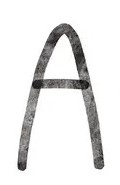
\includegraphics[width=0.6\textwidth]{grayscaleA}
  \caption{This image depicts a Grayscale A to satisfy}
  \label{Fig_grayA} 
  \end{center}
  \end{figure}

\begin{figure}[h!]
  \begin{center}
    
\includegraphics[width=0.6\textwidth]{redA}
  \caption{This image depicts a Red A to satisfy}
  \label{Fig_redA} 
  \end{center}
  \end{figure}

\begin{figure}[h!]
  \begin{center}
    
\includegraphics[width=0.6\textwidth]{greenA}
  \caption{This image depicts a Green A}
  \label{Fig_greenA} 
  \end{center}
  \end{figure}

\begin{figure}[h!]
  \begin{center}
    
\includegraphics[width=0.6\textwidth]{blueA}
  \caption{This image depicts a Blue A}
  \label{Fig_blueA} 
  \end{center}
  \end{figure}

\begin{figure}[h!]
  \begin{center}
    
\includegraphics[width=0.6\textwidth]{Blank_image}
  \caption{This is a blank image}
  \label{Fig_blank} 
  \end{center}
  \end{figure}

\begin{figure}[h!]
  \begin{center}
    
\includegraphics[width=0.6\textwidth]{abc_image}
  \caption{This image depicts the characters A, B and C}
  \label{Fig_ABC} 
  \end{center}
  \end{figure}

\begin{figure}[h!]
  \begin{center}
    
\includegraphics[width=0.6\textwidth]{trainA}
  \caption{This image depicts a sample character from the EMNIST data set used for training and testing the OAR model \citep{EMNIST}}
  \label{Fig_trainA} 
  \end{center}
  \end{figure}
    

\subsection{Understandability Survey Questions} \label{survey_understand}

\begin{itemize}
  \item{On a scale from 1 to 10, how easy was it to understand the code?}
  \item{Were there any OAR specific functions or variable names that caused confusion?}
  \item{Were there any parts of the code that seemed not useful or uneccessary?}
  \item{What part of the code was the most confusing/unclear?}
  \item{Was the use of comments adequate?}
  \item{Do you think you understand the code enough to be able to build upon it further?}
  \item{Would you consider using the software as a learning or teaching tool?}
  \item{Do you have any extra comments or thoughts you'd like to share?}
\end{itemize}

\subsection{Duck Test Checklist} \label{checklist_duckTest}

\begin{itemize}
  \item{Does the code follow a consistent style?}
  \item{Are there any variables that should not be global?}
  \item{Are function names not too long (i.e. less than 40 characters)?}
  \item{Are most functions well named and clear in what they do?}
  \item{Are there any long lines of that can be split into multiple lines?}
  \item{Are global variables and functions documented?}
  \item{Is each function modular (not too long and sufficiently broken down to accomplish a single task)?}
  \item{Are comments plentiful, and written in a way that makes it easy for beginners to follow?}
  \item{Is the code sorted into separate files where reasonable?}
  \item{Is there any duplicate that code be avoided?}
  \item{Is there any use of jargon, domain-specific, or unclear terms?}
  \item{Is all of the code reachable?}
  \item{Is the control flow convoluted?}
  \item{Is there any unnecessarily obscure code? If necessary, is it commented and explained?}
  \item{Could programmer other than the author read the code, and sufficeintly understand it to build upon it?}
  \item{Is there any leftover commented code that is not useful?}
\end{itemize}

\subsection{Usability Survey Questions} \label{survey_useability}

\begin{itemize}
  \item{What operating system do you use?}
  \item{Is OAR running smoothly on your computer?}
  \item{On a scale from 1 to 10, how easy was it to use the software?}
  \item{Was the output of the program satisfactory?}
  \item{What was the least enjoyable feature to use?}
  \item{Was everything legible and clearly displayed? If not, what was not?}
  \item{Would you consider using the software as a learning or teaching tool?}
  \item{Do you have any extra comments or thoughts you'd like to share?}
\end{itemize}

\end{document}